% Project-authored workflow fixture: named nodes, diamond shape, and arrow tips.
\documentclass{article}
\usepackage{tikz}
\usetikzlibrary{arrows.meta,shapes.geometric}

\title{Request Validation Pipeline}
\author{Platform Architecture}
\date{September 2026}

\begin{document}
\maketitle

\section{Ingress checks}
Each incoming request passes schema validation before the service schedules
business logic. Rejected requests return an error without reaching the worker.
The workflow diagram uses named nodes and arrow tips, as a production TikZ
document commonly would.

\begin{figure}
\centering
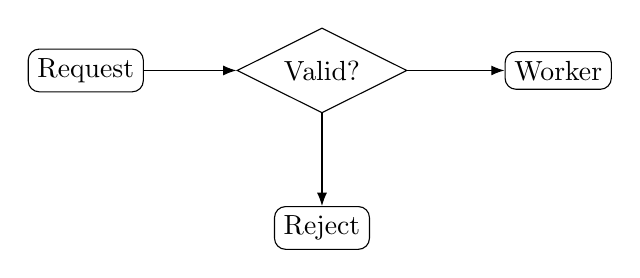
\begin{tikzpicture}
  \node[draw,rounded corners] (request) at (0,0) {Request};
  \node[draw,diamond,aspect=2] (valid) at (3,0) {Valid?};
  \node[draw,rounded corners] (worker) at (6,0) {Worker};
  \node[draw,rounded corners] (reject) at (3,-2) {Reject};
  \draw[-{Latex}] (request) -- (valid);
  \draw[-{Latex}] (valid) -- (worker);
  \draw[-{Latex}] (valid) -- (reject);
\end{tikzpicture}
\caption{Schema validation at the API boundary.}
\label{fig:request-pipeline}
\end{figure}

The branch to the worker handles accepted requests, while rejected requests
follow the downward path. The node labels remain readable inside their shapes.
\end{document}
